\chapter{OTIMIZAÇÃO GLOBAL DOS PARÂMETROS DO SRC DE AFASTAMENTO NULO COM VERY FAST SIMULATED ANEELING}
\label{cap3:vfsa}

O algoritmo Simulated Annealing (SA) é baseado na teoria física da formação de cristais
através do resfriamento lento (Annealing) destes cristais, a partir do seu ponto de fusão \cite{ingber}.
O objetivo do algoritmo é minimizar a função objeto $f(p)$ a patir de perturbações aleatórias do vetor de parâmetros $p$,
para uma nova posição $p'$. O valor $p'$ é avaliado a partir do seguinte critério de aceitação:

\begin{equation}
\label{eq:3.1}
 \Delta f=f(p')-f(p) < 0
\end{equation}

O algoritmo inicia através da escolha de um valor inicial de temperatura, $T=T_0$, para esse valor inicial há
a escolha aleatória do vetor de parâmetros $p_i=(p_1,p_2,p_3,...,p_n)$. O vetor de parâmetros é perturbado 
de sua posição inicial a uma nova posição $p'_i$. Calcula-se o valor da função objeto, $f(p)$ e $f(p')$. Se $f(p')$ é
menor que $f(p)$ significa que o valor da função objeto é menor para o vetor $p'_i$
e a função objeto está convergindo para um mínimo. $p'_i$ é adotado como o
novo vetor de parâmetros, repete-se o processo até atingir o mínimo Global.

Se a Equação \ref{eq:3.1} é satisfeita o valor de $p'$ é aceito como o novo vetor de parâmetros $p$ e o processo
é reiniciado: Perturba-se $p$ para uma nova posição $p'$, e é avaliado se a Equação \ref{eq:3.1} permanece satisfeita. 
Ou seja, a cada nova
iteração a função objeto deverá possuir um valor menor, até que atinja o seu valor mínimo.

Todavia, a função $f(p)$ pode não convergir para o mínimo global, de modo a se manter presa
em um mínimo local. Para tanto, o algoritmo SA permite deslocamentos ascendentes no valor de $f(p)$ a partir de um critério
probabilístico (Critério de Metrópolis): Se $f(p')$ for maior que $f(p)$, a Equação \ref{eq:3.1} não será satisfeita, então
a nova posição $p'$ não será aceita de imediato, devendo passar por um novo teste.

Primeiro, calculamos um número $P$, dado por:

\begin{equation}
\label{eq:3.2}
 P=exp(\frac{-\Delta f}{T})
\end{equation}

E adotamos o seguinte critério probabilístico: 
Se $P$ for maior do que $u$, um número aleatório entre 0 e 1, $p'_i$ será aceito, senão $p'_i$ é
descartado e o algoritmo é reiniciado com uma nova perturbação ao vetor $p$.
Valores baixos de $T$ e altos $\Delta f$ diminuem a probabilidade de que $p'_i$ seja aceito.

O algoritmo Very
Fast Simulated Annealing (VFSA) surgiu com o objetivo de melhorar o desempenho do algoritmo Simulated Annealing (SA). 
Este algoritmo, também é chamado de \textit{Boltzmann Annealing} (BA) e
introduz varias modificações ao
algoritmo padrão SA \cite{ingber}.

No algoritmo VFSA a perturbação de cada elemento $\alpha_{k,i}$ na dimensão $i$ , é realizada
segundo a relação \cite{klaus}:

\begin{equation}
\label{eq:3.3}
 \alpha_{k+1,i}=\alpha_{k,i}+y_i(B_i-A_i)
\end{equation}

Onde $\alpha_{k+1,i}$ é um novo parâmetro obtido a partir do parâmetro $\alpha_{k,i}$ da iteração anterior.
O novo parâmetro é restrito a janela:

\begin{equation}
\label{eq:3.4}
  \alpha_{k+1,i},\alpha_{k,i}\in[A_i,B_i]
\end{equation}

Ou seja, $A_i$ e $B_i$ delimitam o espaço de busca dos parâmetros através da otimização global. 
$u_i$ e $y_i$ são números aleatórios distribuídos da seguinte forma:

\begin{equation}
\label{eq:3.5}
  y_i\in[-1,1]
\end{equation}

\begin{equation}
\label{eq:3.6}
  u_i\in[0,1]
\end{equation}

O cálculo de $y_i$ é dado por:

\begin{equation}
\label{eq:3.7}
  y_i=sgn(u_i-1/2)T_i[(1+1/T_i)^{2u_i-1}-1]
\end{equation}

Onde $sgn()$ é a função sinal, definida da seguinte forma:

%\begin{equation}
$$sgn(t)=1, t > 0$$

$$sgn(t)=-1 t < 0$$
%\end{equation}


O mínimo global pode ser obtido usando a sequência de refriamento $T_i$, definida da seguinte forma \cite{ingber}:

\begin{equation}
\label{eq:3.8}
 T_i(k)=T_{0i}exp(-C_ik^{1/n})
\end{equation}

Onde o parâmetro $T_{0i}$ é a temperatura inicial, e $C_i$ é um parâmetro livre para controle do decaimento e ajuste ao
problema \cite{klaus}. O pseudo-código do algoritmo VFSA é apresentado abaixo \cite{stoffa}:

\vspace{\onelineskip} 

% \begin{algorithm}[H]
% \Entrada{Inicia com um valor aleatório para o parâmetro $m_0$ com uma energia $E(m_0)$}
% \Saida{Parâmetros $p_i$ otimizados}
% \Inicio{
% inicializa\c{c}\~ao\;
% \Repita{fim do texto}{
% leia o atual\;
% \uIf{entendeu}{
% vá para o próximo\;
% próximo se torna o atual\;}
% \Else{volte ao início da seção\;}
% }
% }
% \caption{O pseudo-código do algoritmo Very Fast Simulated Annealing (VFSA).}
% \end{algorithm}


\begin{algorithm}
 \Entrada{Inicia com um valor aleatório para o parâmetro $m_0$ com uma energia $E(m_0)$}
\Saida{Parâmetros $m_i$ do modelo otimizados}

\Repita{arrefecer a temperatura $T_0$ em $q$ iterações}{

  Obtenha a temperatura $T_q$ desta iteração para $M$ parâmetros:
  
  $T=T_0*\exp(-C_0*q^{M^-1});$

    \Repita{atualizar todos os parâmetros do modelo $m_i=1,...,M$}{

      Obtenha um número aleatório $u_i \in U[0,1]$\;

      Obtenha a perturbação do parâmetro $y_i=sgn(u_i-\frac{1}{2})T_i'[(1+T_i')^{2u_i-1}-1]$\;

      Perturbe o parâmetro dentro da janela de busca:

      $m_{new}=m_{old}+y_i(m_{max}-m_{min})$\;

      $m_{min}<=m_{new}<=m_{max}$\;}

    Com os novos parâmetros do modelo ($m_{new}$), calcule o delta da função Energia:
    
    $\Delta E=E(m_{new})-E(m_0)$\;
    
    \Se{$E(m_{new})>E(m_0)$}{
    Guarde os parâmetros atuais ($m_{new}$)\;}

    Para atualizar utilize o critério probabilístico de aceitação (critério de Metropolis):
    
    $P=exp(\frac{-\Delta E}{T})$\;

    \Se{ $\Delta E <= 0$}{
      Atualize:
      
      $m_0=m_{new}$\;

      $E(m_0)=E(m_{new})$\;}

    \Se{ $\Delta E > 0$}{
      Escreva um numero aleatório $r=U[0,1]$\;

      \Se{ $P > 0$}{
	Atualize:
	
	$m_0=m_{new}$\;

	$E(m_0)=E(m_{new})$\;}

    }

}
\caption{O pseudo-código do algoritmo Very Fast Simulated Annealing (VFSA).}
\end{algorithm}

\vspace{\onelineskip} 

\begin{figure}[htb]
\caption{Fluxo de processamento do algoritmo de otimização global Very Fast Simulated Aneeling (VFSA)
proposto para obtenção dos parâmetros do SRC de afastamento nulo.}
\begin{center}
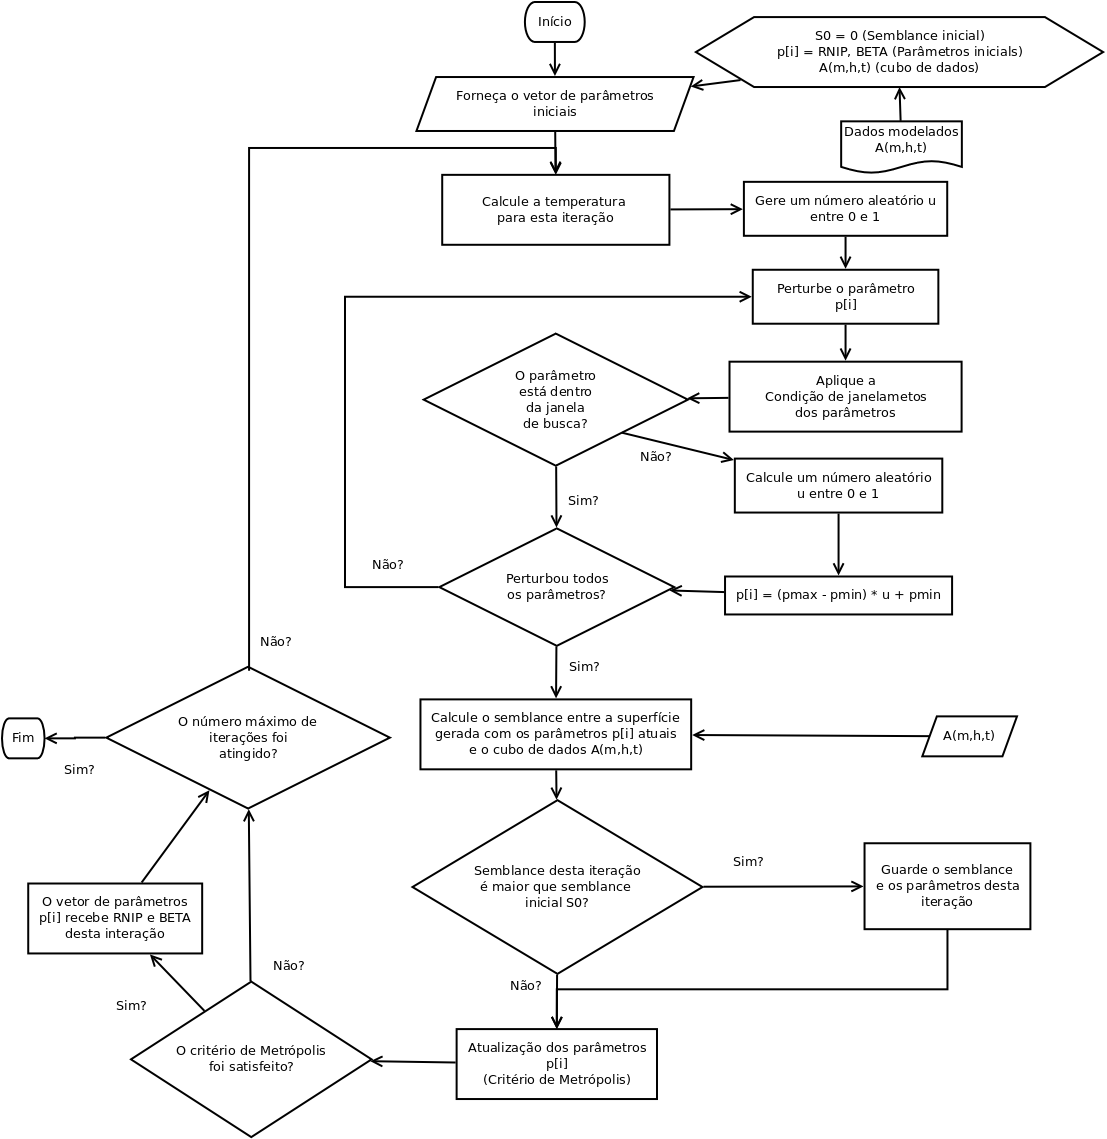
\includegraphics[scale=0.45]{images/VFSA.png}
\vspace{-0.3cm}
\end{center}
\begin{center}
 Fonte: Do Autor.
\end{center}
\label{fig:3.1}
\end{figure}

Podemos utilizar o semblance (coerência) no algoritmo VFSA como critério de convergência na Equação \ref{eq:3.1}
para determinar os parâmetros do SRC $R_N$, $R_{NIP}$ e $\beta_0$. Os dois últimos parâmetros são utilizados também 
no método ERC.

Utilizando uma aproximação de tempo de trânsito SRC, medimos a coerência entre esta aproximação e os
dados no domínio $m, h$, para uma tripla $R_N$, $R_{NIP}$ e $\beta_0$.
A coerência será máxima quando o ajuste entre a aproximação de tempo de trânsito e os dados
for a melhor possível, os parâmetros do SRC que produzirem o melhor ajuste serão o resultado da otimização.

O semblance é uma medida de coerência baseada na soma da energia de traços adjacentes, se os traços alinhados são similares,
a soma dos traços adjacentes será máxima. A definição matemática de semblance para um grupo de $M$ traços, ao 
longo de uma janela de $N$ amostras, na posição $x_j$ e no tempo $t_i$, é dada por \cite{seg}:

\begin{equation}
\label{eq:3.9}
 S_{NM}=\frac{ \sum_{i=1}^N [\sum_{j=1}^M x_j(t_i)]}{M \sum_{i=1}^N \sum_{j=1}^Mx^2_{j}}
\end{equation}

O semblance é a energia da soma dos valores dos traços dividida pela soma da energia dos traços. 
Seu valor máximo é 1 e o mínimo é 0 \cite{seg}. O semblance é medido em uma janela em $m, h$ entre os dados adiquiridos 
e uma superfície de tempo de
trânsito SRC aproximada. 

O Semblance entre a superfície de tempo de trânsito ERC (Equação \ref{eq:2.3})
ou entre a superfície de tempo de trânsito SRC não hiperbólica com condição SDC (Equação \ref{eq:2.4}) 
e os dados modelados é utilizado no critério de
convergência do algoritmo do VFSA Equação \ref{eq:3.1} em cada iteração. 
Os parâmetros $R_N$, $R_{NIP}$ e $\beta_0$ que melhor
ajustam as superfícies aproximadas aos dados serão os parâmetros ótimos.